\section{Introduction}
\label{sec:introduction}

\DeclareFixedFootnote{\youbot-store}{\href{http://www.youbot-store.com}{www.youbot-store.com}}
Models and simulation tools are crucial in robotic research. 
Although there have been major improvements in the electronic and mechanical field, robots are still expensive equipments. 
The use of models and simulation tools overcome this problem.
Models and simulation tools allow researchers and university students to experiment with different robots. 
Furthermore, experimentation with models is cost-efficient and time-efficient due to its ability to be automated, conditioned and accelerated.

The \emph{youBot} is a mobile manipulator designed to serve as the reference platform for industry, research and education \cite{Bischoff2011}.
%Similar to Fraunhofer IPAs Care-O-bot\textregistered \cite{Graf2009} and Willow Garages PR2 \cite{Bohren2011}.
%In practice, the youBot has been equipped with an additional laser scanner or 3D camera sensor.
Due to its frequent use as a test subject for educational purpose or investigation of new methods in research institute, a model of the youBot is highly advantageous. 
Robotic simulation tools which has a model of the youBot are VREP \cite{Freese2010}, We-bots \cite{Michel2004} and Gazebo \cite{Koenig2004}.
Like most robotic simulation software, these software focus on simulating the robot interaction with its surrounding environment (navigation, object manipulation) and have its limitation when simulating the robot's internal components (mechanical, electrical, and control system).
Modeling the robot's internal component requires multi-domain capability such as provided by the Modelica\footnote{\href{https://www.modelica.org
}{www.modelica.org}} description language.
Modelica is a non-proprietary, object-oriented, description language for multi domain modeling.
Modelica is maintained by the non-profit Modelica association.
As such, Modelica is suitable for use in education and research. 
The work in this paper is influenced by the existing manipulator model in the Modelica Standard Library or MSL \cite{Elmqvist1999}.

The youBot standard configuration consists of an omnidirectional mobile platform and a five DOFs manipulator with a two finger gripper.
In this paper, the manipulator model is developed by dividing the system into several smaller components.
The component models are stored in a new Modelica library and categorized in different packages based on its functionality.
This approach enables the user to experiment with the manipulator model on the component level.
\begin{comment}
\begin{figure}[htb]
	\centering
	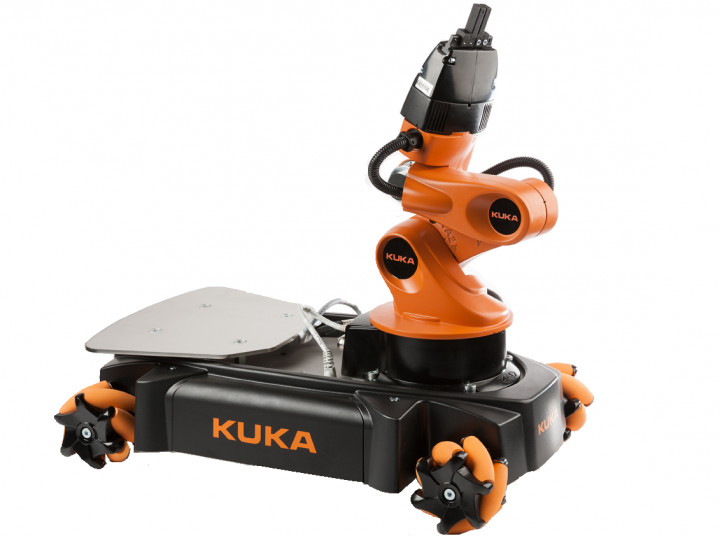
\includegraphics[height=4.4cm]{images/youBot-image.png}
	\caption{Image of youBot\youbot-store}
	\label{fig:youbot}
\end{figure}
\end{comment}

A model is a representation of the actual system and the benefit of having a model only holds true when the model is accurate.
Simulation can result in wrong conclusion when the researcher forget the limitations and condition under which the simulation is valid \cite{Fritzson2004}.
Therefore, the development of the manipulator model is followed by a test with the actual system.
The test compares the behaviors of the actual system and the model throughout a point-to-point motion.
The model accuracy along with the influence of estimated values and approximation is analyzed in the comparison test.

This paper is organized as follows. 
After this introductory section, Modelica related robotic research is presented in Section \ref{sec:state_of_the_art}.
Section \ref{sec:the-youbot-manipulator} presents the specification of the youBot manipulator and Section \ref{sec:the_modelica_package_youbot} describes the Modelica Library for the youBot manipulator. 
Afterward, section \ref{sec:result} presents the evaluation of the developed model.
Finally, section \ref{sec:Conclusion} summarizes the work and provides possible future work.